\documentclass[border=10pt]{standalone}
\usepackage[utf8]{inputenc}
\usepackage[T1]{fontenc}
\usepackage{tikz}
\usetikzlibrary{shapes.geometric, arrows.meta, positioning, fit, backgrounds, calc, shadows}

\begin{document}

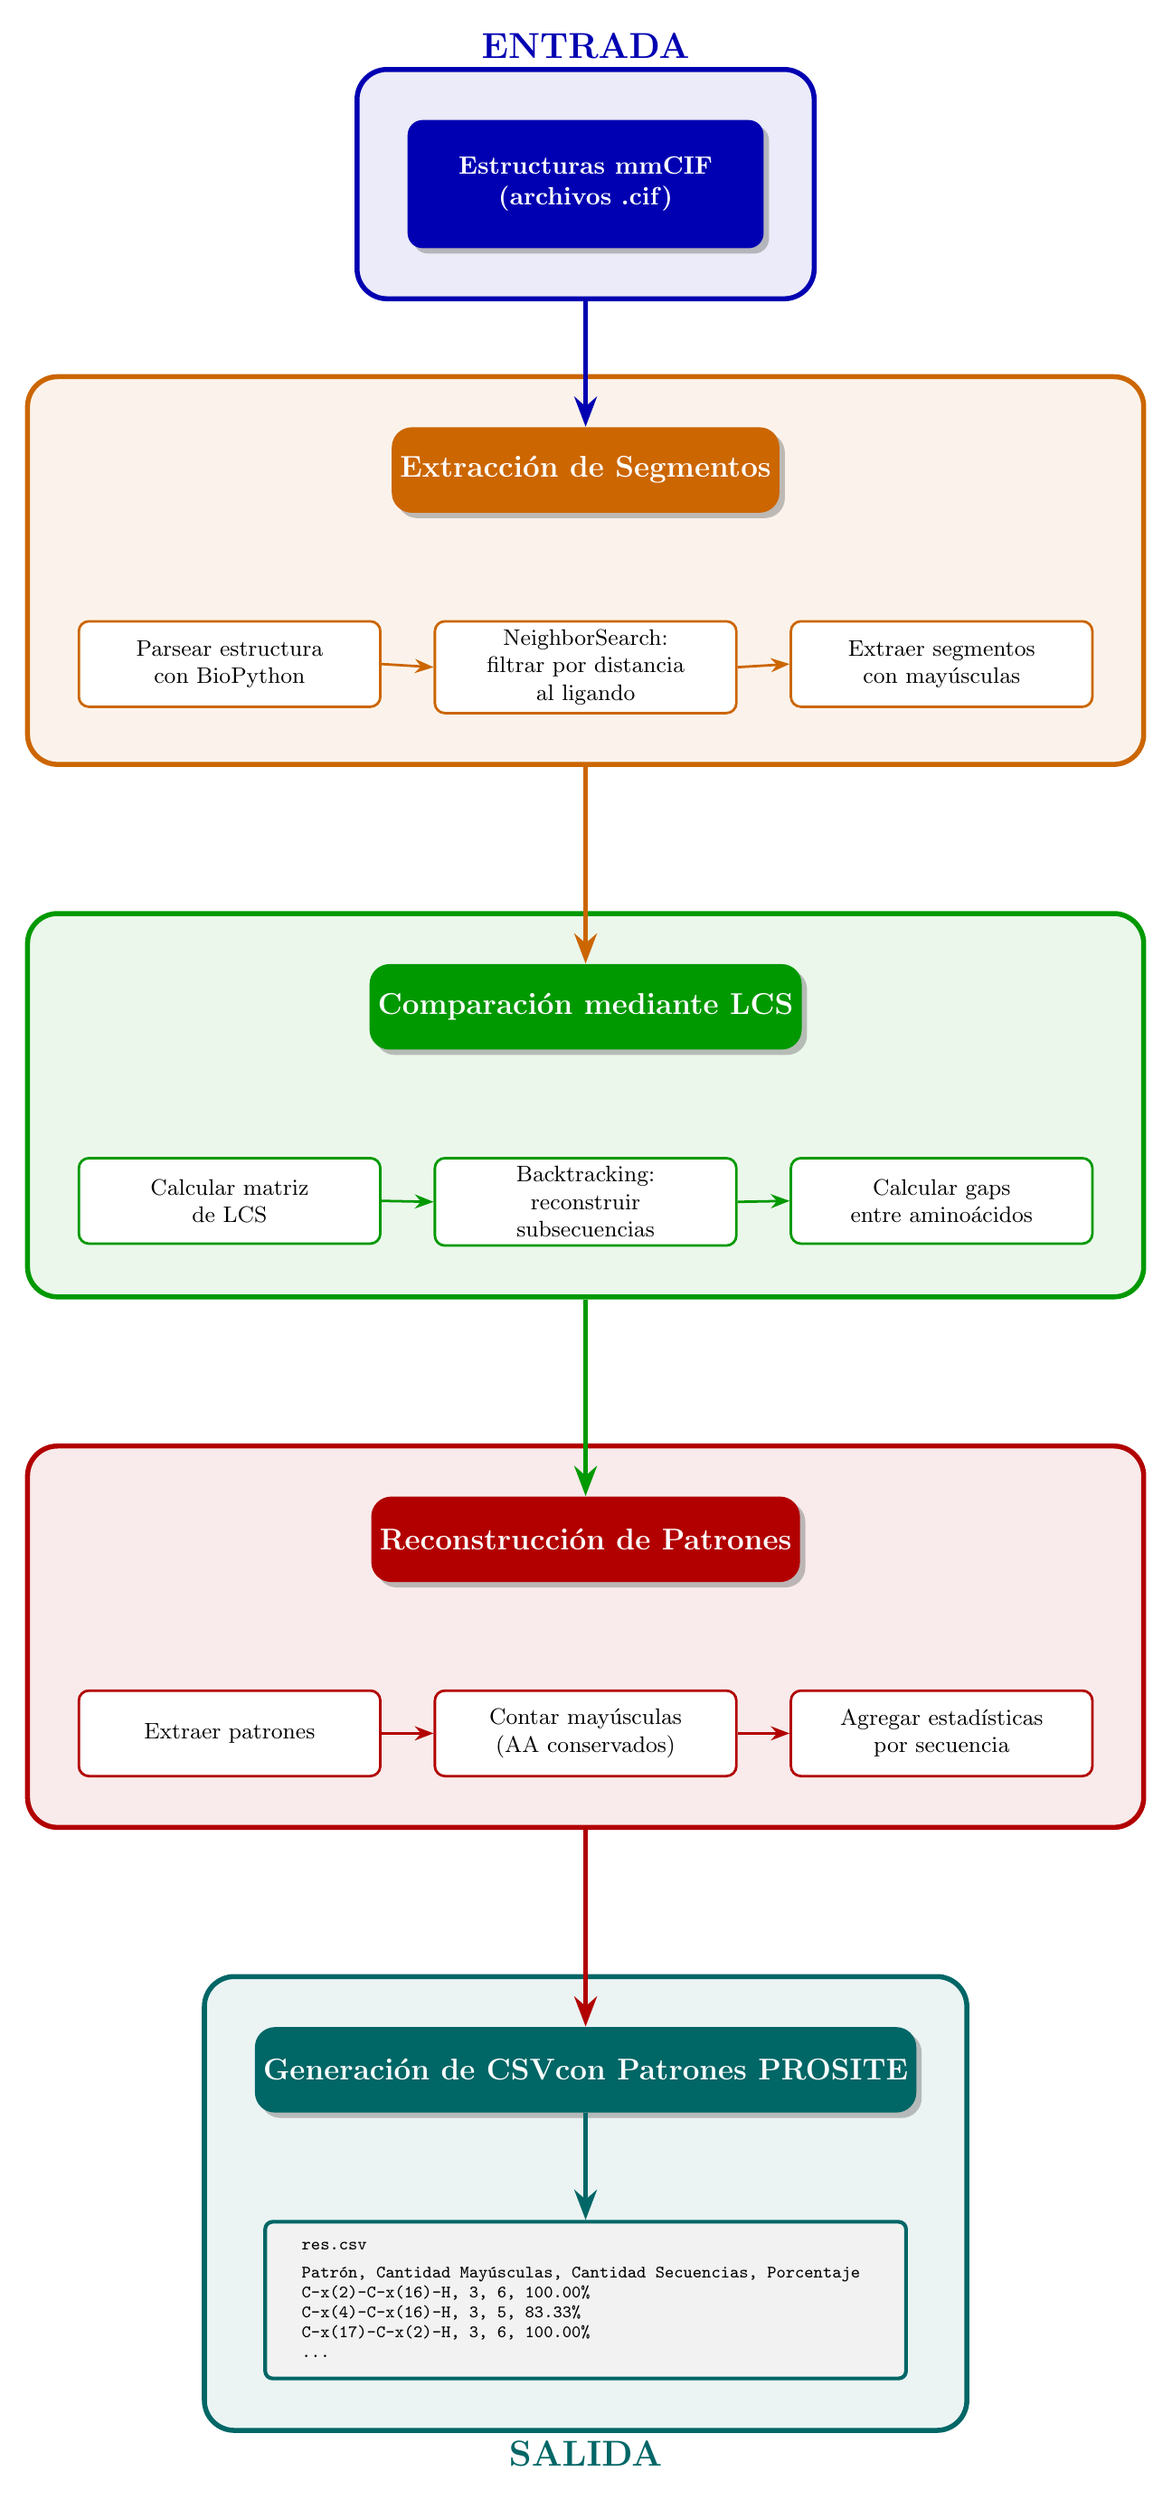
\begin{tikzpicture}[
        node distance=1.5cm and 2cm,
        % Estilos para nodos principales
        mainbox/.style={
                rectangle,
                rounded corners=8pt,
                minimum width=5cm,
                minimum height=1.2cm,
                text centered,
                font=\bfseries\large,
                text=white,
                drop shadow
            },
        % Estilos para sub-nodos
        subbox/.style={
                rectangle,
                rounded corners=4pt,
                minimum width=4.2cm,
                minimum height=1.2cm,
                text centered,
                text width=4cm,
                font=\small,
                text=black,
                fill=white,
                draw=#1,
                line width=1pt
            },
        % Estilo para entrada
        inputbox/.style={
                rectangle,
                rounded corners=6pt,
                minimum height=1.8cm,
                minimum width=5cm,
                text centered,
                text width=4.5cm,
                font=\bfseries,
                text=white,
                fill=blue!70!black,
                drop shadow
            },
        % Estilo para archivo CSV
        csvfile/.style={
                rectangle,
                rounded corners=3pt,
                minimum width=9cm,
                minimum height=2.2cm,
                text centered,
                font=\ttfamily\scriptsize,
                text=black,
                fill=gray!10,
                draw=teal!80!black,
                line width=1.5pt,
                align=left
            },
        % Flechas
        arrow/.style={
                ->,
                >=Stealth,
                line width=2pt,
                color=#1
            },
        % Grupo contenedor
        groupbox/.style={
                rectangle,
                rounded corners=12pt,
                draw=#1,
                line width=2pt,
                fill=#1!8,
                inner sep=15pt
            }
    ]

    % ============================================
    % ENTRADA
    % ============================================
    \node[inputbox] (pdb) {Estructuras mmCIF\\(archivos .cif)};

    % Grupo de entrada
    \begin{scope}[on background layer]
        \node[groupbox=blue!70!black, fit=(pdb), inner sep=20pt, label={[font=\bfseries\Large, text=blue!70!black]above:ENTRADA}] (entrada) {};
    \end{scope}

    % ============================================
    % EXTRACCIÓN DE AMINOÁCIDOS (Interactions.py)
    % ============================================
    \node[mainbox, fill=orange!80!black, below=2.5cm of pdb] (extraccion) {Extracción de Segmentos};

    \node[subbox=orange!80!black, below=1.5cm of extraccion, xshift=-5cm] (ext1) {Parsear estructura\\con BioPython};
    \node[subbox=orange!80!black, below=1.5cm of extraccion] (ext2) {NeighborSearch:\\filtrar por distancia\\al ligando};
    \node[subbox=orange!80!black, below=1.5cm of extraccion, xshift=5cm] (ext3) {Extraer segmentos\\con mayúsculas};

    % Grupo extracción
    \begin{scope}[on background layer]
        \node[groupbox=orange!80!black, fit=(extraccion)(ext1)(ext2)(ext3), inner sep=20pt] (gext) {};
    \end{scope}


    % ============================================
    % COMPARACIÓN LCS (batchcompare + patternfinder)
    % ============================================
    \node[mainbox, fill=green!60!black, below=3.5cm of ext2] (comparacion) {Comparación mediante LCS};

    \node[subbox=green!60!black, below=1.5cm of comparacion, xshift=-5cm] (comp1) {Calcular matriz\\de LCS};
    \node[subbox=green!60!black, below=1.5cm of comparacion] (comp2) {Backtracking:\\reconstruir\\subsecuencias};
    \node[subbox=green!60!black, below=1.5cm of comparacion, xshift=5cm] (comp3) {Calcular gaps\\entre aminoácidos};

    % Grupo comparación
    \begin{scope}[on background layer]
        \node[groupbox=green!60!black, fit=(comparacion)(comp1)(comp2)(comp3), inner sep=20pt] (gcomp) {};
    \end{scope}

    % ============================================
    % RECONSTRUCCIÓN DE PATRONES
    % ============================================
    \node[mainbox, fill=red!70!black, below=3.5cm of comp2] (reconstruccion) {Reconstrucción de Patrones};

    \node[subbox=red!70!black, below=1.5cm of reconstruccion, xshift=-5cm] (rec1) {Extraer patrones};
    \node[subbox=red!70!black, below=1.5cm of reconstruccion] (rec2) {Contar mayúsculas\\(AA conservados)};
    \node[subbox=red!70!black, below=1.5cm of reconstruccion, xshift=5cm] (rec3) {Agregar estadísticas\\por secuencia};

    % Grupo reconstrucción
    \begin{scope}[on background layer]
        \node[groupbox=red!70!black, fit=(reconstruccion)(rec1)(rec2)(rec3), inner sep=20pt] (grec) {};
    \end{scope}

    % ============================================
    % SALIDA - CSV con patrones PROSITE
    % ============================================
    \node[mainbox, fill=teal!80!black, below=3.5cm of rec2] (traduccion) {Generación de CSV\\con Patrones PROSITE};

    \node[csvfile, below=1.5cm of traduccion] (csv) {
        \begin{tabular}{l}
            \textbf{res.csv}                                             \\[3pt]
            Patrón, Cantidad Mayúsculas, Cantidad Secuencias, Porcentaje \\
            C-x(2)-C-x(16)-H, 3, 6, 100.00\%                             \\
            C-x(4)-C-x(16)-H, 3, 5, 83.33\%                              \\
            C-x(17)-C-x(2)-H, 3, 6, 100.00\%                             \\
            ...
        \end{tabular}
    };

    % Grupo salida
    \begin{scope}[on background layer]
        \node[groupbox=teal!80!black, fit=(traduccion)(csv), inner sep=20pt, label={[font=\bfseries\Large, text=teal!80!black]below:SALIDA}] (salida) {};
    \end{scope}

    % ============================================
    % FLECHAS PRINCIPALES
    % ============================================
    \draw[arrow=blue!70!black] (entrada.south) -- (extraccion.north);

    \draw[arrow=orange!80!black] (gext.south) -- ++(0,-0.6) -- (comparacion.north);
    \draw[arrow=green!60!black] (gcomp.south) -- ++(0,-0.6) -- (reconstruccion.north);
    \draw[arrow=red!70!black] (grec.south) -- ++(0,-0.6) -- (traduccion.north);
    \draw[arrow=teal!80!black] (traduccion.south) -- (csv.north);

    % Flechas entre sub-nodos
    \draw[arrow=orange!80!black, line width=1pt] (ext1.east) -- (ext2.west);
    \draw[arrow=orange!80!black, line width=1pt] (ext2.east) -- (ext3.west);

    \draw[arrow=green!60!black, line width=1pt] (comp1.east) -- (comp2.west);
    \draw[arrow=green!60!black, line width=1pt] (comp2.east) -- (comp3.west);

    \draw[arrow=red!70!black, line width=1pt] (rec1.east) -- (rec2.west);
    \draw[arrow=red!70!black, line width=1pt] (rec2.east) -- (rec3.west);

\end{tikzpicture}

\end{document}
